\documentclass[a4paper]{scrreprt}
 
\usepackage[english]{babel}
\usepackage[utf8]{inputenc}
\usepackage[T1]{fontenc}
\usepackage{ae}
\usepackage[bookmarks,bookmarksnumbered]{hyperref}
\usepackage{graphicx}
\newsavebox{\mybox}
\newenvironment{user-story}[1]{\begin{lrbox}
		{\mybox}\begin{minipage}[t]{5in}\begin{center}\begin{minipage}[t]{5in}\begin{description}\item[{ID: }] #1 \label{ustory:#1}}
		{\end{description}\end{minipage}\end{center}\end{minipage}\end{lrbox}\fbox{\usebox{\mybox}}} 

\begin{document}
 
\title{Functional specification document for fpga-design-re GUI}
\author{Sebastian Wallat \\
		\texttt{sebastian.wallat@rub.de}
		}
\maketitle
 
\tableofcontents
 
\chapter{Target acquisition}
The purpose of this chapter is the definition of target without specifying the required functions to implement the targets.
 
\section{Mandatory ('must') criteria}
This section enumerates the required functions of the final product. These are imperative functions that are needed in the final product. The system is without these criteria not usable for the desired purpose.

\begin{enumerate}
  \item Graphical view of data model
  \item Plugin executable
  \item Plugin effect visible in Graphic view
  \item Textview (Nodes \& Edges)
  \item Items Selectable
  \item Source View
  \item Color sync different views
\end{enumerate}

 
\section{Optional ('should') criteria}
The fulfillment of the following criteria is desirable but not mandatory. The implementation of these criteria should be intended if enough capacities are available.

\begin{enumerate}
  \item Color specification of plugins
  \item Grouping of items
  \item Selection model for graphical and standard views
  \item Project information files
  \item Search for node/edge type or specific information
  \item Syntax highlighting VHDL
  \item Miniview in file
  \item Line numbers text view
  \item Tabbed view
  \item Keyboard shortcuts
\end{enumerate}

 
\section{Distinction criteria}
The following criteria are explicitly intended not to be fulfilled.
 
\chapter{Product application}
In this chapter the environment and boundary conditions are specified.

\section{Area of application}
The final GUI should be used in laboratory and open source environments. 

\section{Target audiences}
The main audience are hardware reverse engineers and cryptanalysts, who are trying to reproduce and modify a given netlist and produce a synthesizeable file format.
 
\section{Operating conditions}
This section should define the physical constraints of the system. Such conditions are daily usage time, the information if the system is under steady observation by an operator or weather an unattended use is intended.

\begin{description}
  \item[attended or unattended] The GUI is intended to be used attended only.
  \item[number of parallel netlists] The GUI is intended to operate on one netlist at a time.
\end{description}

 
\chapter{Environment}
 
\section{Software}
Which software needs to be available to use the specified system. Libraries and version numbers.

\begin{description}
  \item[OS] The development is mainly done on a Apple MacBook Pro. Beside Mac OS X 10.10 support for Linux (Ubuntu LTS) and basic support for Windows 10 should be provided.
  \item[Qt 5.5] The basic graphic framework used is Qt 5.5. Here mainly the widget framework is used.
\end{description}

 
\section{Hardware}
The supported input and output platform for netlists is Xilinx Spartan 6.

\chapter{Product overview}

Figure \ref{img:context} depicts the system context.

\begin{figure}[hbt]
  \centering
  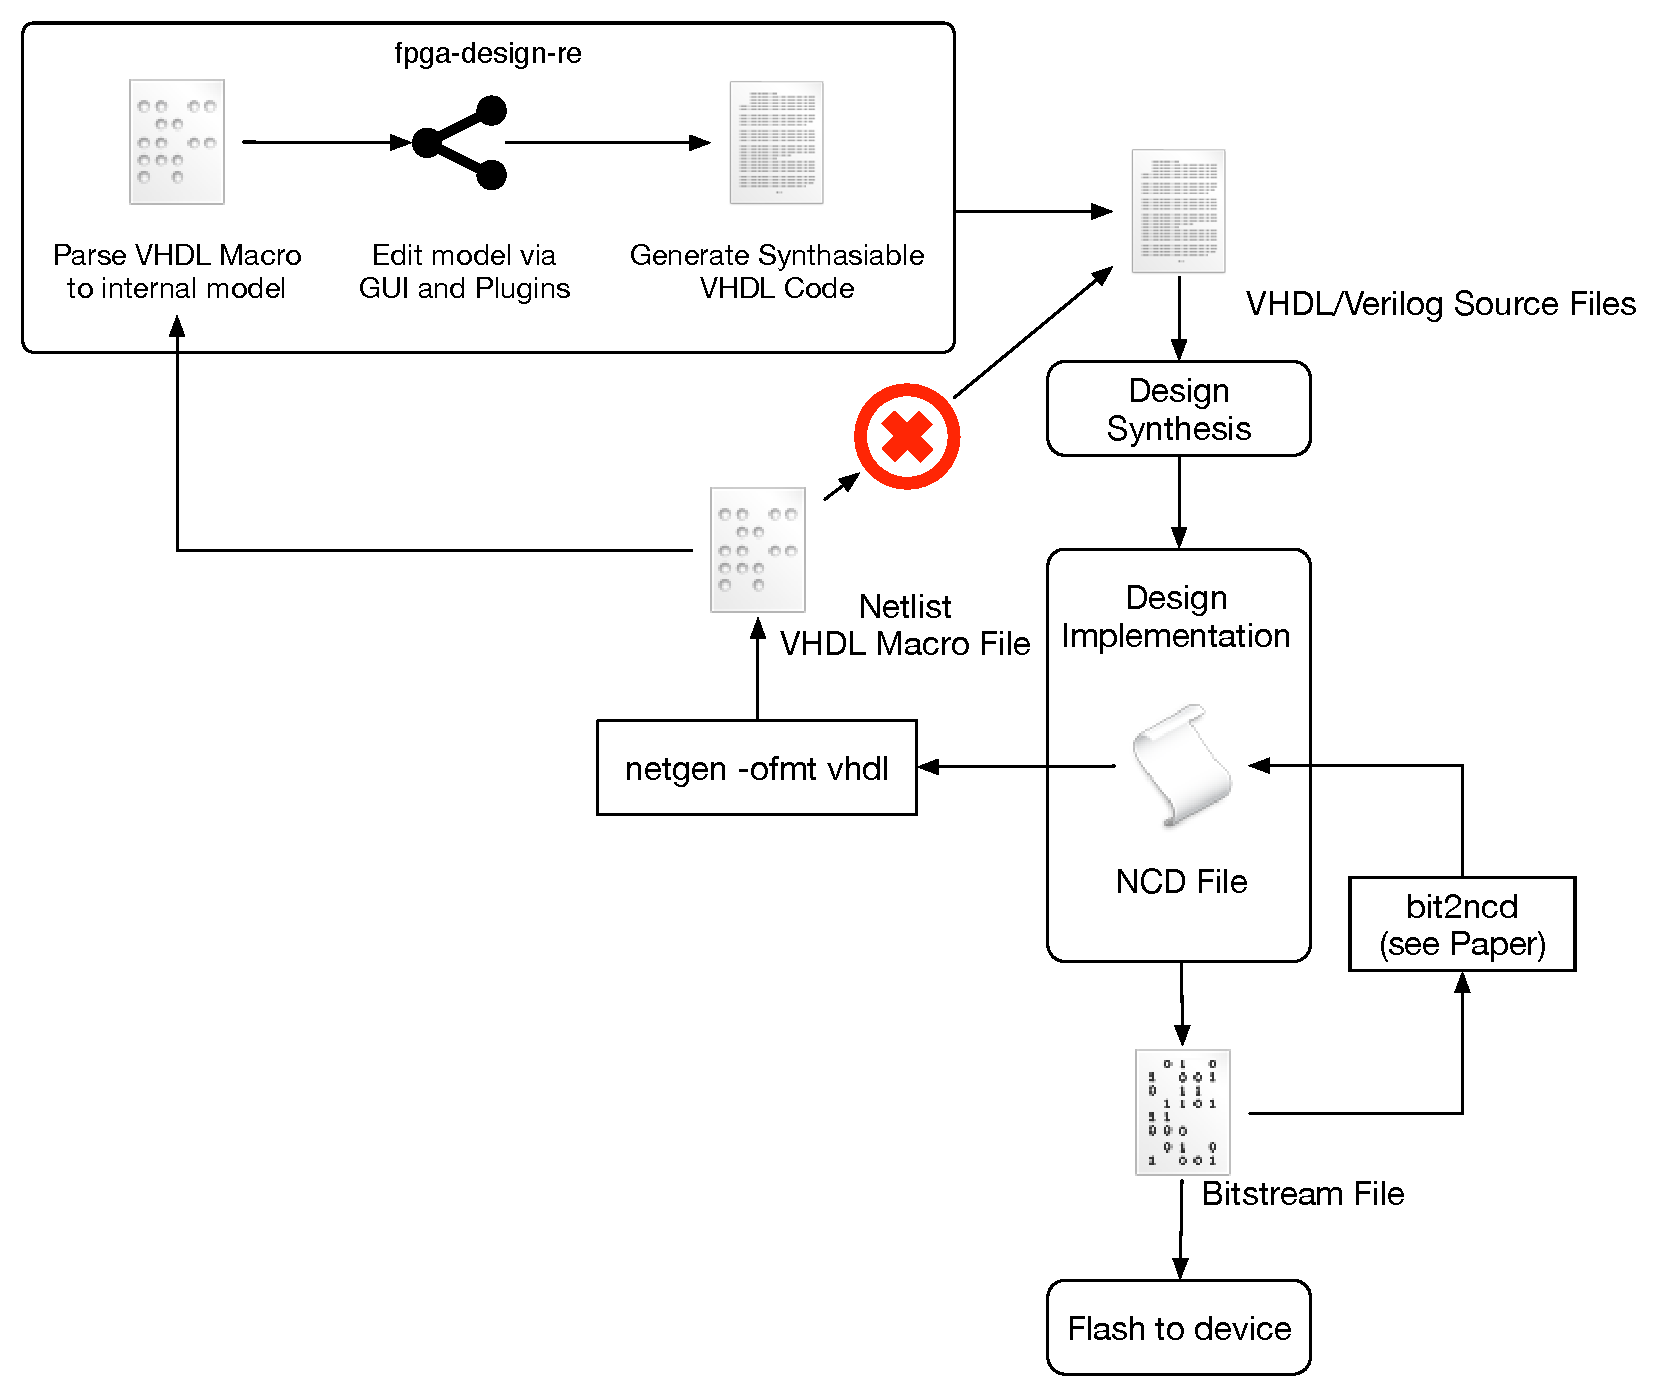
\includegraphics[scale=0.5]{images/Processes}
  \caption{System Context}
  \label{img:context}
\end{figure}
\newpage
\section{GUI}

\begin{figure}[hbt]
  \centering
  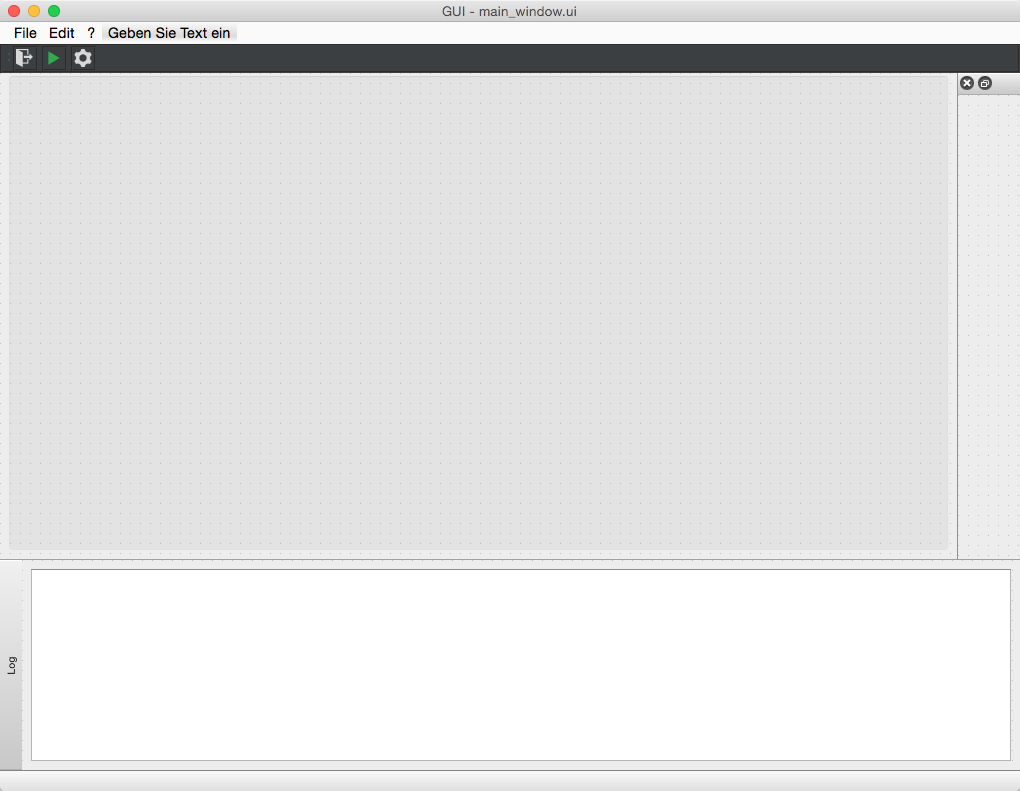
\includegraphics[scale=0.4]{images/main_window_ui}
  \caption{Main Window UI}
  \label{img:main-win}
\end{figure}

\begin{figure}[hbt]
  \centering
  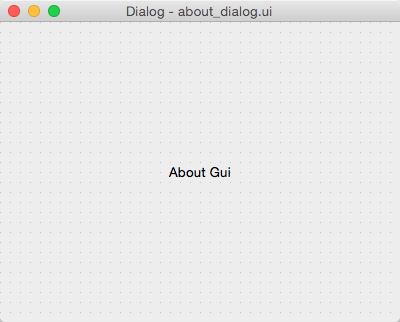
\includegraphics[scale=0.5]{images/about_dialog_ui}
  \caption{About Dialog}
  \label{img:about-diag}
\end{figure}


\begin{figure}[hbt]
  \centering
  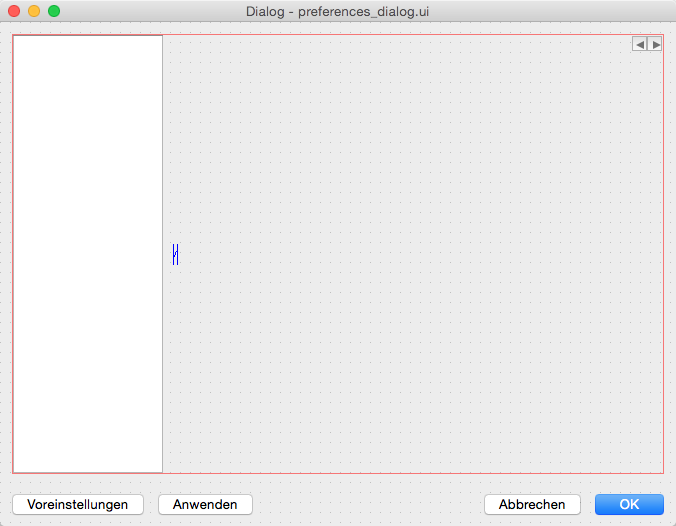
\includegraphics[scale=0.5]{images/preference_dialog_ui}
  \caption{Preferences Dialog}
  \label{img:pref-dialog}
\end{figure}

\begin{figure}[hbt]
  \centering
  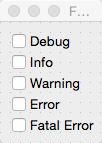
\includegraphics[scale=0.5]{images/logger_settings_widget_ui}
  \caption{Logger preferences widget}
  \label{img:logger-widget}
\end{figure}

\begin{figure}[hbt]
  \centering
  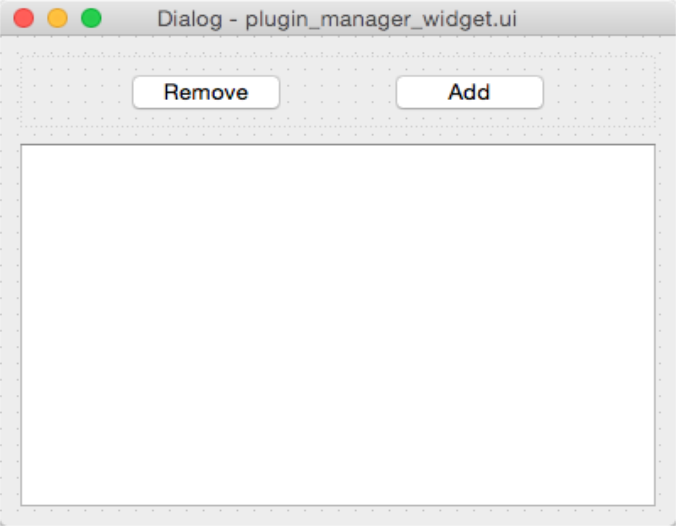
\includegraphics[scale=0.5]{images/plugin_manager_widget_ui}
  \caption{Plugin manager widget}
  \label{img:plugin-widget}
\end{figure}

 
%\chapter{Functional specification}
%This chapter specifies the specific product functionalities which includes a detailed description. 
% 
%\begin{itemize}
%  \item typical operating cycles
%  \item No definition of typical management functions (CRUD) \footnote{Create,
%Read, Update, Delete}
%\end{itemize}
%
%%%%% PATTERN TO COPY
%%% ref to story: \ref{ustory:<ID>}
%%\begin{user-story}{<ID>}
%%	\item[{Actors: }]
%%	\item[{Pre-condition: }]
%%	\item[{Trigger Event: }]
%%	\item[{Story: }] In order to <receive benefit> as a <role>, I want <goal/desire>
%%	\item[{Expected behaviour: }]
%%	\item[{Post-conditions: }] 
%%	\item[{Exceptions: }]	
%%\end{user-story}
%
%\begin{user-story}{user-story-sample}
%	\item[{Actors: }]
%	\item[{Pre-condition: }]
%	\item[{Trigger Event: }]
%	\item[{Story: }] In order to <receive benefit> as a <role>, I want <goal/desire>
%	\item[{Expected behaviour: }]
%	\item[{Post-conditions: }] 
%	\item[{Exceptions: }]	
%\end{user-story}

\chapter{Data}
This chapter should described the pieces of information that are needed to be saved persistently.

\begin{itemize}
  \item Json file(s) - internal data model
  \item Input file
  \item Synthezisable output file
\end{itemize}

 
%\chapter{Perfomance}
%This chapter specifies performance requirement like used time and accuracy. Here should be noted, that these should be quantifiable requirements.
% 
%\chapter{Quality requirements}
%This chapter specifies targets for quality aspect of the product. These requirements should be objectively quantifiable, specific and relevant. Requirements that are only subjectively quantifiable are not intended to be specified.

%\chapter{Amendments}
%This chapter presents additional intformation.
 

\listoffigures
 
\end{document}